\documentclass[a4paper]{article}

\usepackage[pages=all, color=black, position={current page.south}, placement=bottom, scale=1, opacity=1, vshift=5mm]{background}
\usepackage[margin=1in]{geometry} % full-width

% AMS Packages
\usepackage{amsmath}
\usepackage{amsthm}
\usepackage{amssymb}
\usepackage{natbib}  % Add the natbib package for citations
%\usepackage{biblatex}
% Unicode
\usepackage[utf8]{inputenc}
\usepackage[hidelinks]{hyperref}

\hypersetup{
	unicode,
%	colorlinks,
%	breaklinks,
%	urlcolor=cyan, 
%	linkcolor=blue, 
	pdfauthor={Author One, Author Two, Author Three},
	pdftitle={Sentiment Classification},
	pdfsubject={Sentiment Classification},
	pdfkeywords={article, template, simple},
	pdfproducer={LaTeX},
	pdfcreator={pdflatex}
}

% Vietnamese
%\usepackage{vntex}

% Natbib
\usepackage[sort&compress,numbers,square]{natbib}

% Theorem, Lemma, etc
\theoremstyle{plain}
\newtheorem{theorem}{Theorem}
\newtheorem{corollary}[theorem]{Corollary}
\newtheorem{lemma}[theorem]{Lemma}
\newtheorem{claim}{Claim}[theorem]
\newtheorem{axiom}[theorem]{Axiom}
\newtheorem{conjecture}[theorem]{Conjecture}
\newtheorem{fact}[theorem]{Fact}
\newtheorem{hypothesis}[theorem]{Hypothesis}
\newtheorem{assumption}[theorem]{Assumption}
\newtheorem{proposition}[theorem]{Proposition}
\newtheorem{criterion}[theorem]{Criterion}
\theoremstyle{definition}
\newtheorem{definition}[theorem]{Definition}
\newtheorem{example}[theorem]{Example}
\newtheorem{remark}[theorem]{Remark}
\newtheorem{problem}[theorem]{Problem}
\newtheorem{principle}[theorem]{Principle}

\usepackage{caption}  % Customize caption settings
\usepackage{lipsum}   % Example package for dummy text

\usepackage{graphicx, color}
\graphicspath{{fig/}}
\captionsetup[figure]{justification=raggedright,singlelinecheck=false}
%\usepackage[linesnumbered,ruled,vlined,commentsnumbered]{algorithm2e} % use algorithm2e for typesetting algorithms
\usepackage{algorithm, algpseudocode} % use algorithm and algorithmicx for typesetting algorithms
\usepackage{mathrsfs} % for \mathscr command

\usepackage{lipsum}

% Author info

\title{\textbf{Sentiment Classification using ML Algorithms}}
\author{
    \begin{tabular}{@{\hspace{2cm}}l r}
        Mahek Vanjani & (B22EE088) \\
        Vidhi Jain & (B22CS083) \\
        Himanshu Sharma & (B22EE080)\\
        Priyansh Saxena & (B22EE075) \\
        Vasishtha Pandya & (B22CS036) \\
        Anushka Desai & (B22EE012) \\
        Saumya Shah & (B22CS074)
    \end{tabular}
}
\begin{document}
	\maketitle
	\begin{abstract}
The study of public opinion can provide us with valuable information. The analysis of sentiment on social networks, such as Twitter or Facebook, has become a powerful means of learning about users’ opinions and has a wide range of applications. In this study, we utilized traditional machine learning models including decision trees, logistic regression, k-nearest neighbors (KNN), support vector machines (SVM), as well as ensemble methods such as bagging and boosting. These models were applied to analyze sentiment and extract insights from social media data.
\vspace{0.2 cm}\newline
In addition to the machine learning models mentioned, we employed the NLTK (Natural Language Toolkit) library for text processing tasks. We conducted experiments comparing models with and without NLTK(Natural Language Tool Kit) preprocessing. Furthermore, our analyses incorporated term frequency-inverse document frequency (TF-IDF) and word embedding techniques applied to multiple datasets. These approaches enabled comprehensive exploration of sentiment analysis methods and their effectiveness in understanding public opinion expressed on social media platforms.
\vspace{0.2 cm}\newline
		\noindent\textbf{Keywords:} sentiment analysis;machine learning; natural language processing\vspace{0.3 cm}
	\end{abstract}\hrule{}

	\tableofcontents \vspace{1 cm}
	\hrule{}
	\section{Introduction}
	\label{sec:intro}
The landscape of social interaction has been transformed by platforms such as blogs, forums, and social media, which serve as digital hubs for global communication and information sharing. This user-generated content reflects originality and provides valuable opinions essential for applications ranging from personalized recommendations to political strategies. Analyzing sentiments expressed in this vast volume of text is now essential, facilitated by AI-driven techniques like sentiment analysis powered by deep neural networks. However, capturing the intricacies of human emotions, including nuances like sarcasm and context, remains a complex challenge for these algorithms.

In the realm of web-based companies, understanding customer sentiment towards products requires sophisticated sentiment analysis techniques that go beyond simplistic keyword matching. Machine learning advancements, especially with deep neural networks, have greatly improved the accuracy of sentiment analysis, enabling a more nuanced understanding of textual emotions. This technology plays a crucial role in extracting actionable insights from large-scale user opinions, facilitating informed decision-making and enhancing customer experience strategies.
\vspace{0.3 cm}
\hrule{}
\section{Background}
	\label{sec:app}
In traditional machine learning approaches, features are defined and extracted either manually
or by making use of feature selection methods. Figure below shows the
sentiment polarity classification through traditional machine learning (Support
Vector Machine (SVM), Bayesian networks, or decision trees etc.) . Several types of machine learning
techniques are discussed in this section.
\begin{figure}[htbp] % Placement options (h=here, t=top, b=bottom, p=page)
    % \raggedleft
    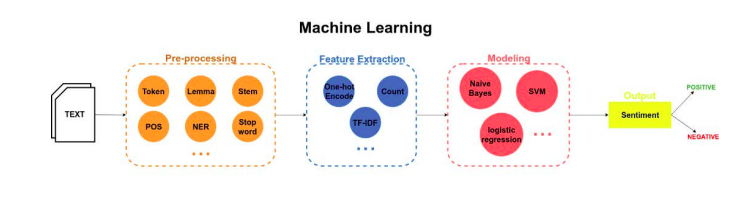
\includegraphics[width=1\textwidth]{figs/ml.png} % Replace 'figs/new.jpg' with your image file path
    % \caption{Machine}
    \label{fig:example}
\end{figure}

2.1.1 \textbf{Naive Bayes Classifier\newline}

Naïve Bayes classifiers work differently in that they operate under a couple of key assumptions, earning it the title of “naïve”. It assumes that predictors in a Naïve Bayes model are conditionally independent, or unrelated to any of the other feature in the model. It also assumes that all features contribute equally to the outcome. While these assumptions are often violated in real-world scenarios (e.g. a subsequent word in an e-mail is dependent upon the word that precedes it), it simplifies a classification problem by making it more computationally tractable. That is, only a single probability will now be required for each variable, which, in turn, makes the model computation easier. Despite this unrealistic independence assumption, the classification algorithm performs well, particularly with small sample sizes.\newline

2.1.2 \textbf{Support Vector Machine (SVM) \newline}

SVMs are commonly used within classification problems. They distinguish between two classes by finding the optimal hyperplane that maximizes the margin between the closest data points of opposite classes. The number of features in the input data determine if the hyperplane is a line in a 2-D space or a plane in a n-dimensional space. Since multiple hyperplanes can be found to differentiate classes, maximizing the margin between points enables the algorithm to find the best decision boundary between classes. This, in turn, enables it to generalize well to new data and make accurate classification predictions. The lines that are adjacent to the optimal hyperplane are known as support vectors as these vectors run through the data points that determine the maximal margin.

The SVM algorithm is widely used in machine learning as it can handle both linear and nonlinear classification tasks. However, when the data is not linearly separable, kernel functions are used to transform the data higher-dimensional space to enable linear separation. This application of kernel functions can be known as the “kernel trick”, and the choice of kernel function, such as linear kernels, polynomial kernels, radial basis function (RBF) kernels, or sigmoid kernels, depends on data characteristics and the specific use case.\newline

\begin{figure}[htbp] % Placement options (h=here, t=top, b=bottom, p=page)
    % \raggedleft
    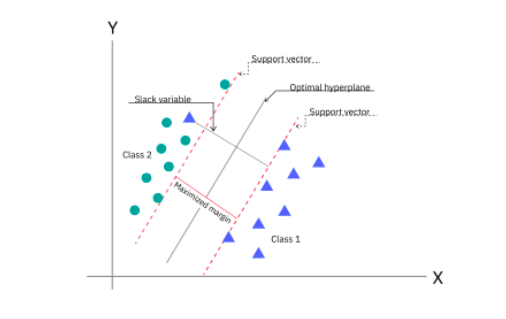
\includegraphics[width=1\textwidth]{figs/SVM.png} % Replace 'figs/new.jpg' with your image file path
    % \caption{This is a caption describing the figure.}
    \label{fig:example}
\end{figure}\newline

2.1.3 \textbf{Logistic Regression\newline}

This type of statistical model (also known as logit model) is often used for classification and predictive analytics. Since the outcome is a probability, the dependent variable is bounded between 0 and 1. In logistic regression, a logit transformation is applied on the odds—that is, the probability of success divided by the probability of failure. This is also commonly known as the log odds, or the natural logarithm of odds, and this logistic function is represented by the following formulas: \newline

Logit(pi) = 1/(1+ exp(-pi))\newline

ln(pi/(1-pi)) = Beta_0 + Beta_1*X_1 + … + B_k*K_k\newline

In this logistic regression equation, logit(pi) is the dependent or response variable and x is the independent variable. The beta parameter, or coefficient, in this model is commonly estimated via maximum likelihood estimation (MLE). This method tests different values of beta through multiple iterations to optimize for the best fit of log odds. All of these iterations produce the log likelihood function, and logistic regression seeks to maximize this function to find the best parameter estimate. Once the optimal coefficient (or coefficients if there is more than one independent variable) is found, the conditional probabilities for each observation can be calculated, logged, and summed together to yield a predicted probability. For binary classification, a probability less than .5 will predict 0 while a probability greater than 0 will predict 1.  After the model has been computed, it’s best practice to evaluate the how well the model predicts the dependent variable, which is called goodness of fit. The Hosmer–Lemeshow test is a popular method to assess model fit.\newline

2.1.4\textbf{ Decision Tree Classifier\newline}

Decision tree learning employs a divide and conquer strategy by conducting a greedy search to identify the optimal split points within a tree. This process of splitting is then repeated in a top-down, recursive manner until all, or the majority of records have been classified under specific class labels. Whether or not all data points are classified as homogenous sets is largely dependent on the complexity of the decision tree. Smaller trees are more easily able to attain pure leaf nodes—i.e. data points in a single class. However, as a tree grows in size, it becomes increasingly difficult to maintain this purity, and it usually results in too little data falling within a given subtree. When this occurs, it is known as data fragmentation, and it can often lead to overfitting. As a result, decision trees have preference for small trees, which is consistent with the principle of parsimony in Occam’s Razor; that is, “entities should not be multiplied beyond necessity.” Said differently, decision trees should add complexity only if necessary, as the simplest explanation is often the best. To reduce complexity and prevent overfitting, pruning is usually employed; this is a process, which removes branches that split on features with low importance. The model’s fit can then be evaluated through the process of cross-validation. Another way that decision trees can maintain their accuracy is by forming an ensemble via a random forest algorithm; this classifier predicts more accurate results, particularly when the individual trees are uncorrelated with each other.\newline

\begin{figure}[htbp] % Placement options (h=here, t=top, b=bottom, p=page)
    % \raggedleft
    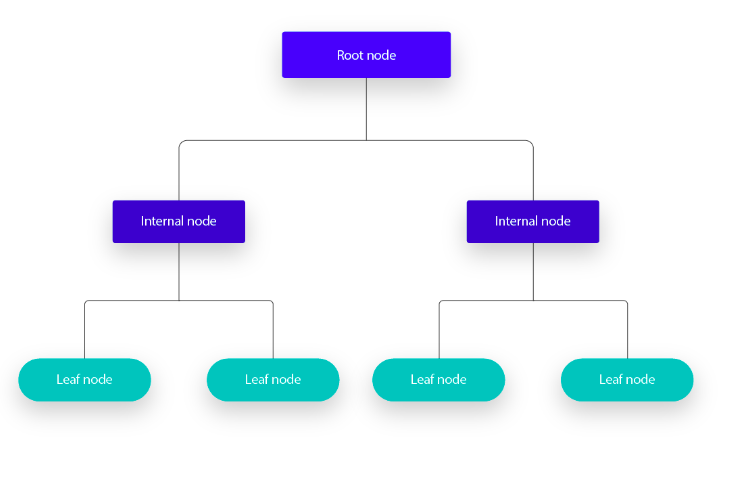
\includegraphics[width=0.7\textwidth]{figs/decisiontree.png} % Replace 'figs/new.jpg' with your image file path
    % \caption{This is a caption describing the figure.}
    \label{fig:example}
\end{figure}\newline

2.1.5 \textbf{Random Forest CLassifier\newline}

The random forest algorithm is an extension of the bagging method as it utilizes both bagging and feature randomness to create an uncorrelated forest of decision trees. Feature randomness, also known as feature bagging or “the random subspace method”(link resides outside ibm.com), generates a random subset of features, which ensures low correlation among decision trees. This is a key difference between decision trees and random forests. While decision trees consider all the possible feature splits, random forests only select a subset of those features.\newline

2.1.6 \textbf{Gradient Boosting Classifier\newline}

Gradient Boosting is a functional gradient algorithm that repeatedly selects a function that leads in the direction of a weak hypothesis or negative gradient so that it can minimize a loss function. Gradient boosting classifier combines several weak learning models to produce a powerful predicting model.\newline

2.1.7\textbf{ AdaBoost Classifier\newline}

AdaBoost algorithm, introduced by Freund and Schapire in 1997, revolutionized ensemble modeling. Since its inception, AdaBoost has become a widely adopted technique for addressing binary classification challenges. This powerful algorithm enhances prediction accuracy by transforming a multitude of weak learners into robust, strong learners

The principle behind boosting algorithms is that we first build a model on the training dataset and then build a second model to rectify the errors present in the first model. This procedure is continued until and unless the errors are minimized and the dataset is predicted correctly. Boosting algorithms work in a similar way, it combines multiple models (weak learners) to reach the final output (strong learners).\newline

2.1.8\textbf{ k-nearest neighbors (KNN)\newline}

The k-nearest neighbors (KNN) algorithm is a non-parametric, supervised learning classifier, which uses proximity to make classifications or predictions about the grouping of an individual data point. It is one of the popular and simplest classification and regression classifiers used in machine learning today.

While the KNN algorithm can be used for either regression or classification problems, it is typically used as a classification algorithm, working off the assumption that similar points can be found near one another.\newline

2.1.9  \textbf{Light Gradient Boosting Machine Classifier\newline}

LightGBM is a powerful and efficient open-source gradient boosting framework for machine learning. It’s specifically designed to handle large datasets and perform well in terms of speed and memory usage. LightGBM uses a technique called gradient boosting, which combines multiple weak learners (usually decision trees) to create a strong predictive model.\newline

\textbf{2.2 Sentiment Analysis\newline}

Sentiment analysis encompasses automatic extraction of subjective information from text to discern whether users' content conveys positive, negative, or neutral sentiments. ML-based techniques for sentiment analysis are categorized into traditional and deep learning models. Traditional methods like the naive Bayes classifier, maximum entropy classifier, and support vector machines (SVM) use lexical and sentiment lexicon-based features for input. In contrast, deep learning models such as CNNs, DNNs, and RNNs excel in sentiment analysis at various levels like the document, sentence, or aspect. Before applying sentiment analysis, text data undergoes preprocessing involving removal of extraneous characters (e.g., white spaces, punctuation), lemmatization to reduce words to their base form, and transformation into numerical vectors via word embedding (e.g., Word2vec) or TF-IDF. These techniques convert raw text data into continuous real-number vectors, enabling effective sentiment analysis tasks ranging from objective or subjective classification to aspect-based analysis.
\vspace{0.2 cm}\newline
ML-driven sentiment analysis finds extensive applications in diverse domains like business intelligence, e-commerce, and healthcare. In business, companies leverage sentiment analysis on customer feedback to enhance customer support, product development, and marketing strategies. Sentiment analysis aids in understanding user opinions on events or products, illuminating industrial trends and informing decision-making. The application extends to recommender systems, where sentiment analysis enhances recommendations based on sentiment analysis of reviews. Moreover, sentiment analysis plays a role in behavioral analysis and commodity markets. In healthcare, sentiment analysis of social media texts contributes to mental health monitoring, complementing or replacing traditional questionnaires with data-driven insights from patient posts.
\newline

\textbf{2.3 Application of Sentiment Analysis}
\newline
It is widely accepted that sentiment analysis is very useful in a wide range of application domains, such as business, government, and biomedicine.
\vspace{0.2 cm}\newline
{Business Intelligence and E-commerce:}
\begin{itemize}
    \item Analyzing customer feedback to support product improvement and marketing strategies.
    \item Understanding public sentiment about events and products to correlate with preferences and habits.
\end{itemize}
\newline
{Recommender Systems:}
\begin{itemize}
    \item Monitoring sentiment analysis along with reviews to enhance recommendations for restaurants, movies, and other services.
\end{itemize}
\newline
{Commodity Markets and Behavioral Analysis:}
\begin{itemize}
    \item Employing sentiment analysis to understand market changes and consumer behavior.
\end{itemize}
\newline
{Biomedicine and Healthcare:}
\begin{itemize}
    \item Utilizing sentiment analysis for opinion mining of health-related texts on social media and blogs.
    \item Creating medical lexicons to aid in symptom and disease description.
    \item Enhancing mental health evaluation by applying sentiment analysis to patient posts alongside conventional questionnaires.
\end{itemize}
\hrule{}
\section{Experiments and Results}
\label{sec:experiments}
\textbf{3.1 Dataset:\newline}
The dataset used for the experiments is in CSV format, with emoticons removed. The data file consists of six fields:

\begin{enumerate}
    \item \textbf{Polarity of the tweet}: This field indicates the sentiment polarity of the tweet.
        \begin{itemize}
            \item 0 = Negative
            \item 1 = Neutral
            \item 2 = Positive
        \end{itemize}
    \item \textbf{Tweet ID}: Unique identifier for the tweet (e.g., 2087).
    \item \textbf{Date of the tweet}: Timestamp indicating when the tweet was posted (e.g., Sat May 16 23:58:44 UTC 2009).
    \item \textbf{Query}: Specifies the query associated with the tweet. If no query is present, the value is set to NO\_QUERY.
    \item \textbf{User}: Username of the Twitter user who posted the tweet (e.g., robotickilldozr).
    \item \textbf{Text of the tweet}: The actual content of the tweet (e.g., "Lyx is cool").(Ref fig 2)
\end{enumerate}
\begin{figure}[htbp]
  \centering
  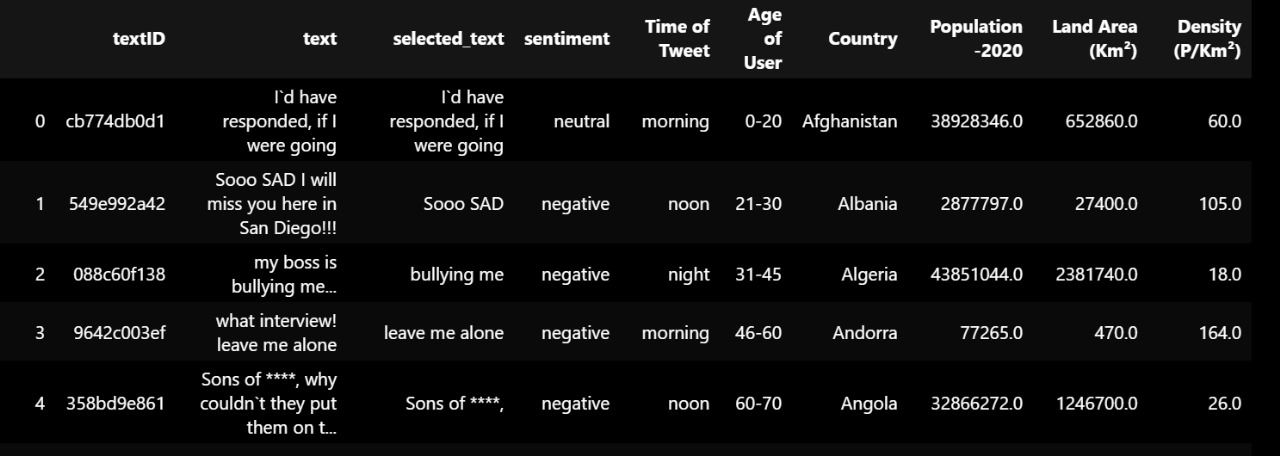
\includegraphics[width=0.7\textwidth]{figs/6.jpg}
  \caption{Example of The Datset}
  \label{fig:confusion_matrix}
\end{figure}


\textbf{3.2 Methodological Approach \& Results:}

After examining the approach outlined in Section 2, we conducted experiments to evaluate the accuracy of various models while comparing the results obtained with and without the use of NLTK (Natural Language Toolkit) for text preprocessing. The goal was to assess the impact of NLTK on model performance in sentiment analysis tasks.\newline
3.2.1 Without NLTK:\vspace{0.2 cm}\newline
3.2.1.1 Text Preprocessing:\newline \begin{itemize}
    \item Applied a custom preprocessing function (\texttt{wp(text)}) to clean and normalize the \texttt{selected\_text} column.
    \item The function handled tasks such as converting text to lowercase, removing special characters, URLs, HTML tags, punctuation, and numeric characters.
\end{itemize}
\newline{Feature Engineering}

\begin{itemize}
    \item Encoded categorical variables (\texttt{sentiment}, \texttt{Time of Tweet}, \texttt{Country}) into numerical codes for model compatibility.
    \item Mapped age groups (\texttt{Age of User}) to approximate integer values to represent user demographics effectively.
\end{itemize}
\newline{Text Vectorization}

\begin{itemize}
    \item Utilized \texttt{TfidfVectorizer} for text vectorization, converting preprocessed text data into TF-IDF numerical representations.
    \item This vectorization process transformed textual data into a format suitable for machine learning model training.
\end{itemize}\newline
3.2.1.2 Models \newline

We implemented multiple machine learning models(discussed in Section 2) for sentiment analysis and evaluated their performance using various metrics.
\begin{table}[htbp]
    \centering
    \caption{Model Performance Metrics}
    \label{tab:model_metrics}
    \begin{tabular}{|l|c|c|c|c|}
        \hline
        \textbf{Model} & \textbf{Accuracy} & \textbf{Precision} & \textbf{Recall} & \textbf{F1-score} \\
        \hline
        Decision Tree(maxdepth=20) & 0.64 & 0.72 & 0.64 & 0.64 \\
        Logistic Regression & 0.83 & 0.84 & 0.82 & 0.83 \\
        Naive Bayes Classifier & 0.77 & 0.84 & 0.75 & 0.77 \\
        K-nearest neighbors(k=5) & 0.51 & 0.67 & 0.57 & 0.48 \\
        Random Forest Classifier & 0.81 & 0.83 & 0.80 & 0.81 \\
        Boosting(AdaBoost Classifier) & 0.69 & 0.73 & 0.70 & 0.70 \\
        Gradient Boosting & 0.74& 0.77 & 0.74 & 0.74 \\
        LightGBM & 0.79 & 0.80 & 0.79 & 0.79 \\
        SVM(kernel=linear) & 0.83 & 0.84 & 0.83 & 0.83 \\
        SVM(kernel=polynomial) & 0.78 & 0.85 & 0.76 & 0.78\\
        SVM(kernel=rbf) & 0.83 & 0.85 & 0.83 & 0.84 \\
        \hline
    \end{tabular}
\end{table}

3.2.1.3 Inference \newline
\begin{itemize}
    \item Logistic Regression emerges as the top-performing model with the highest accuracy (83\%) and balanced precision (84\%) and recall (82\%). This indicates that logistic regression effectively captures the sentiment patterns in the text data and provides reliable predictions.
    \item Support Vector Machines (SVM), particularly with the linear and radial basis function (RBF) kernels, also exhibit competitive performance, achieving accuracies of 83\% and 84\% respectively. SVMs are known for their effectiveness in handling high-dimensional data and complex decision boundaries.
    \item Random Forest Classifier follows closely with an accuracy of 81\%, showcasing its robustness in handling noise and overfitting while maintaining high predictive accuracy.
    \item Naive Bayes Classifier and Gradient Boosting demonstrate respectable performance, suitable for sentiment analysis tasks, although they exhibit slightly lower accuracies compared to logistic regression and SVMs.
    \item K-nearest neighbors (KNN), in this case with $k = 5$, performs relatively weaker compared to other models, suggesting limitations in its ability to generalize well on the sentiment analysis task.
\end{itemize}
3.2.2 With NLTK:\vspace{0.2 cm}\newline
3.2.2.1 Data Preprocessing
\begin{itemize}
    \item {Handling Missing Values}:The dataset is initially cleaned by removing rows containing missing values (NaN).
    \item {Visualizing Sentiment Distribution}:A bar plot is generated to visualize the distribution of sentiments ('positive', 'neutral', 'negative') in the dataset. This helps in understanding the class distribution and potential class imbalance issues.
    \item {Addressing Class Imbalance}:Class imbalance is addressed by downsampling the majority classes ('positive' and 'negative') to match the size of the minority class ('neutral'). This ensures a balanced dataset for training and evaluation.
\end{itemize}

3.2.2.1.2 Text Preprocessing Steps
\begin{itemize}
    \item {Removing Stop Words:} Stop words are removed from the text data using NLTK's predefined list of English stop words to eliminate common words that do not contribute to sentiment analysis.
    \item{Cleaning Text:} Special characters, HTML tags, non-alphabetic characters, and punctuation are removed from the text to focus on meaningful words.
    \item {Lowercasing:} Text is converted to lowercase to ensure consistency in word representations.
    \item {Tokenization and Lemmatization:} Text is tokenized into words and lemmatized to reduce words to their base or root form, which helps in standardizing text features.
\end{itemize} 
\newlne{3.2.2.2 Exploratory Data Analysis (EDA)}
\item{3.2.2.2.1 Word Cloud Visualization}\newline
\begin{itemize}
    \item{Positive Sentiment}:A word cloud visualization highlights prevalent words associated with positive sentiment, such as "thank", "love", "LOL", and "happy".
    \item{Neutral Sentiment}:The word cloud for neutral sentiment indicates a lack of distinct word patterns compared to other sentiments.
    \item{Negative Sentiment}:Negative sentiment is characterized by words like "sad", "tired", "suck", and "sorry", as depicted in the word cloud visualization.(Refer fig 3)
    \end{itemize}
{3.2.2.2.2 Top One-word Counts} \newline
\begin{itemize}
    \item {Positive Sentiment}: Common one-word occurrences in positive sentiment include "good", "day", "thanks", and "great".
    \item {Neutral Sentiment}:Neutral sentiment does not exhibit prominent word patterns based on one-word counts.
    \item {Negative Sentiment}: Key one-word occurrences in negative sentiment involve words like "work", "miss", and "sad".(Fig 4)
\end{itemize}

{3.2.2.2.3 Inference and Observations}
\begin{itemize}
    \item The analysis reveals distinct word usage patterns across different sentiment categories.
    \item Positive sentiment is associated with expressions of positivity and gratitude.
    \item Negative sentiment includes words indicating dissatisfaction and sadness.
    \item Neutral sentiment lacks clear word patterns compared to positive and negative sentiments, making it potentially challenging for classification.
\end{itemize}
3.2.2.2.3 Models \newline

We implemented multiple machine learning models(discussed in Section 2) for sentiment analysis(using NLTK) and evaluated their performance using various metrics.(Refer Table 2)

\begin{table}[htbp]
    \centering
    \caption{Model Performance Metrics}
    \label{tab:model_metrics}
    \resizebox{\textwidth}{!}{%
    \begin{tabular}{lcccccccc}
    \toprule
    \textbf{Model} & \textbf{Training Acc.} & \textbf{Testing Acc.} & \textbf{Avg. Prec.} & \textbf{Avg. Recall} & \textbf{Avg. F1-Score} \\
    \midrule
    Naive Bayes & 0.86 & 0.78 & 0.88 & 0.84 & 0.86 \\
    Linear SVM & 0.93 & 0.80 & 0.85 & 0.81 & 0.83 \\
    Logistic Regression & 0.89 & 0.80 & 0.86 & 0.79 & 0.82 \\
    Decision Tree & 0.98 & 0.77 & 0.93 & 0.77 & 0.83 \\
    Random Forest & 0.98 & 0.80 & 0.90 & 0.80 & 0.85 \\
    Gradient Boosting & 0.70 & 0.68 & 0.80 & 0.65 & 0.68 \\
    AdaBoost & 0.65 & 0.65 & 0.78 & 0.61 & 0.62 \\
    KNN & 0.58 & 0.51 & 0.66 & 0.58 & 0.56 \\
    Poly SVC & 0.97 & 0.76 & 0.93 & 0.67 & 0.78 \\
    RBF SVC & 0.95 & 0.81 & 0.90 & 0.70 & 0.79 \\
    LightGBM & 0.81 & 0.78 & 0.81 & 0.78 & 0.79 \\
    \midrule
 
    \bottomrule
    \end{tabular}%
    }
\end{table}
\newline

3.2.2.2.4 Inference:
\newline

Based on the evaluation of various machine learning models for sentiment analysis, we draw the following conclusions:

\begin{itemize}
  \item \textbf{Naive Bayes:} Naive Bayes achieved a training accuracy of 86\% and testing accuracy of 78\%. The model shows good average precision (88\%) and recall (84\%), resulting in an overall F1-score of 86\%.
  
  \item \textbf{Linear SVM:} The Linear SVM model demonstrates strong generalization performance with a training accuracy of 93\% and testing accuracy of 80\%. It maintains good precision (85\%) and recall (81\%), resulting in an F1-score of 83\%.
  
  \item \textbf{Logistic Regression:} Logistic Regression performs consistently well with a training accuracy of 89\% and testing accuracy of 80\%. It achieves a balanced trade-off between precision (86\%) and recall (79\%), resulting in an F1-score of 82\%.
  
  \item \textbf{Decision Tree:} The Decision Tree model achieves very high training accuracy (98\%) but exhibits lower generalization to unseen data with a testing accuracy of 77\%. Despite high precision (93\%), the model's lower recall (77\%) results in a slightly lower F1-score of 83\%.
  
  \item \textbf{Random Forest:} Random Forest shows robustness against overfitting with consistent performance (training accuracy: 98\%, testing accuracy: 80\%). It maintains high precision (90\%) and recall (80\%), leading to an overall F1-score of 85\%.
  
  \item \textbf{Gradient Boosting:} Gradient Boosting achieves moderate training accuracy (70\%) and testing accuracy (68\%), indicating a degree of underfitting. The model's precision (80\%) and recall (65\%) result in a balanced F1-score of 68\%.
  
  \item \textbf{AdaBoost:} AdaBoost demonstrates the lowest performance among the models, with training and testing accuracies of 65\%. It exhibits lower precision (78\%) and recall (61\%), resulting in an overall F1-score of 62\%.
  
  \item \textbf{KNN:} KNN performs relatively poorly compared to other models, with training accuracy of 58\% and testing accuracy of 51\%. The model's precision (66\%) and recall (58\%) result in a low F1-score of 56\%.
  
  \item \textbf{Poly SVC and RBF SVC:} Both SVM models (Poly and RBF) achieve high training accuracies (97\% and 95\%, respectively) but slightly lower testing accuracies (76\% and 81\%, respectively). They maintain high precision (93\% and 90\%) and recall (67\% and 70\%), resulting in balanced F1-scores of 78\% and 79\%, respectively.
  
  \item \textbf{LightGBM:} LightGBM demonstrates moderate performance with training accuracy of 81\% and testing accuracy of 78\%. It achieves balanced precision (81\%) and recall (78\%), resulting in an F1-score of 79\%.
\end{itemize}
Random Forest achieved the highest F1-score (85\%) and demonstrated robustness against overfitting, outperforming other models. Linear SVM and Logistic Regression also showed strong performance with balanced precision and recall.
\vspace{0.3 cm}
\hrule{}
\section{Summary}
\label{sec:app}

The project aimed to evaluate the effectiveness of different machine learning models for sentiment analysis, comparing results with and without the use of NLTK (Natural Language Toolkit) for text preprocessing. Here are the key findings of the study:

\textbf{Results:}

\textbf{Without NLTK:}
\begin{itemize}
    \item Logistic Regression was the top-performing model with 83\% accuracy and balanced precision and recall.
    \item SVM (linear and RBF kernels) demonstrated competitive performance.
    \item Random Forest showed robustness against overfitting with an 81\% F1-score.
\end{itemize}

\textbf{With NLTK:}
\begin{itemize}
    \item Naive Bayes achieved an 86\% F1-score, indicating improved performance with NLTK preprocessing.
    \item Linear SVM and Logistic Regression maintained strong performance with text preprocessing.
\end{itemize}
\textbf{
Observations:}
\begin{itemize}
    \item NLTK-based analysis revealed distinct word patterns for positive, negative, and neutral sentiments.
    \item Random Forest emerged as the top-performing model overall, highlighting its effectiveness in sentiment analysis tasks.
    \item NLTK preprocessing significantly enhanced the performance of certain models, particularly Naive Bayes.
\end{itemize}
\section{Figures}
\begin{figure}[htbp]
% First row: Two figures side by side
    \begin{minipage}[b]{0.45\textwidth}
        \centering
        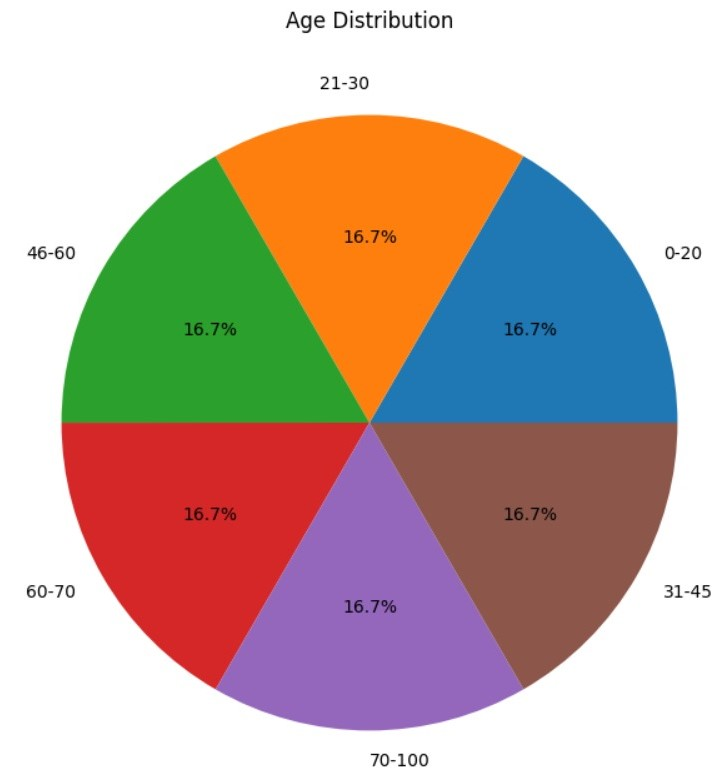
\includegraphics[width=\textwidth]{figs/1.jpg}
        \caption*{Age Distribution for Tweets in twitter}
        \label{fig:figure1}
    \end{minipage}
    \hfill
    \begin{minipage}[b]{0.45\textwidth}
        \centering
        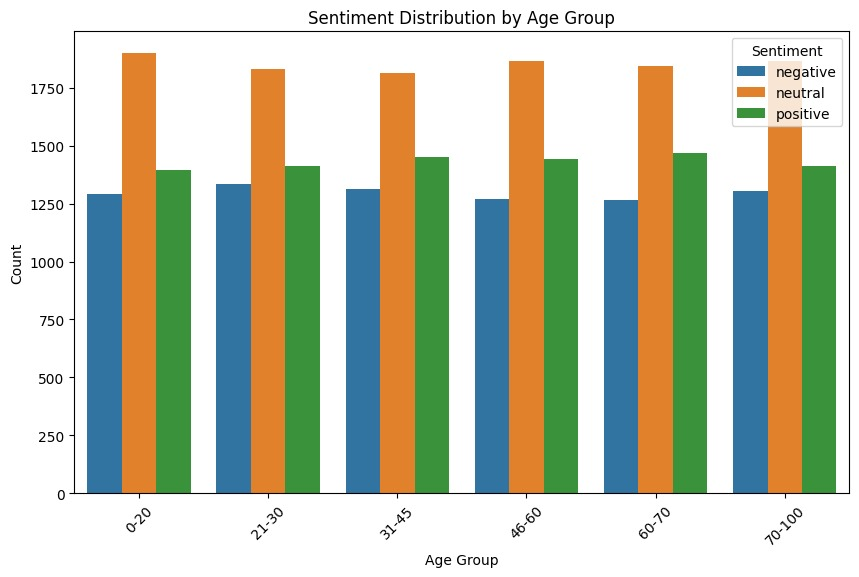
\includegraphics[width=\textwidth]{figs/2.jpg}
        \caption*{Sentiment Distribution by Age Group}
        \label{fig:figure2}
    \end{minipage}
    
    \vspace{\baselineskip} % Add some vertical space
    
    % Second row: Three figures
    \begin{minipage}[b]{0.3\textwidth}
        \centering
        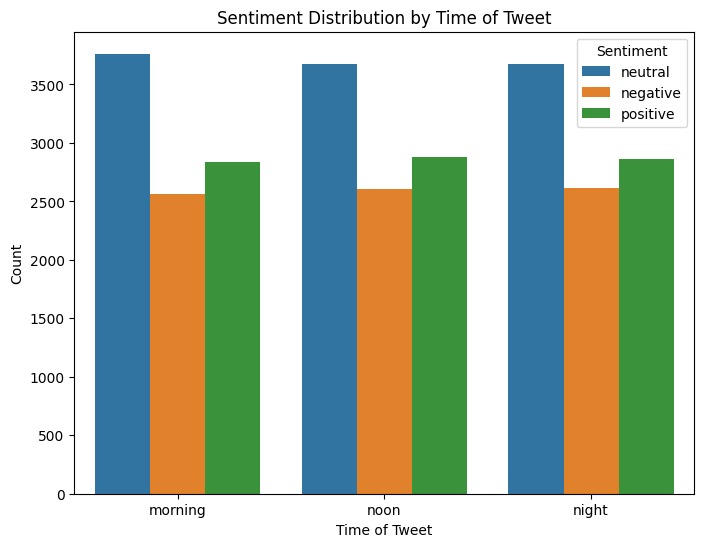
\includegraphics[width=\textwidth]{figs/3.jpg}
        \caption*{Sentiment Distribution v/s Time of Tweet}
        \label{fig:figure3}
    \end{minipage}
    \hfill
    \begin{minipage}[b]{0.3\textwidth}
        \centering
        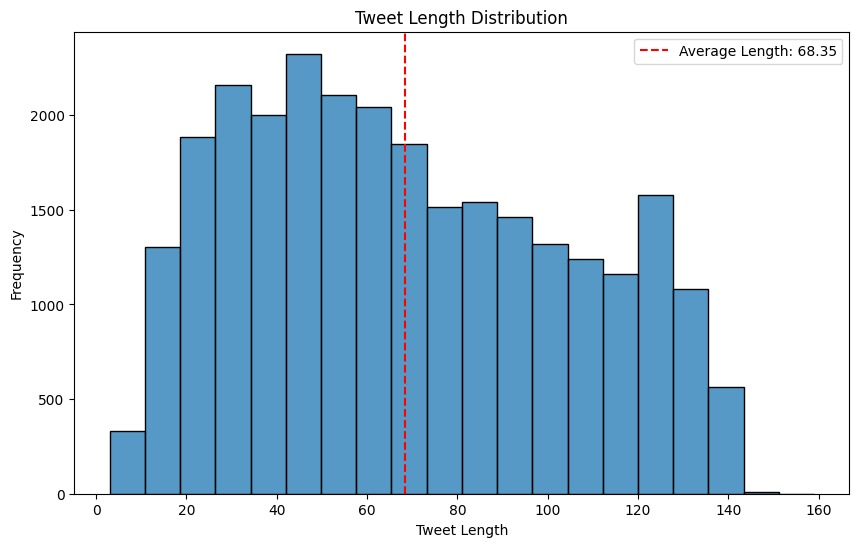
\includegraphics[width=\textwidth]{figs/4.jpg}
        \caption*{Average Tweet Length }
        \label{fig:figure4}
    \end{minipage}
    \hfill
    \begin{minipage}[b]{0.3\textwidth}
        \centering
        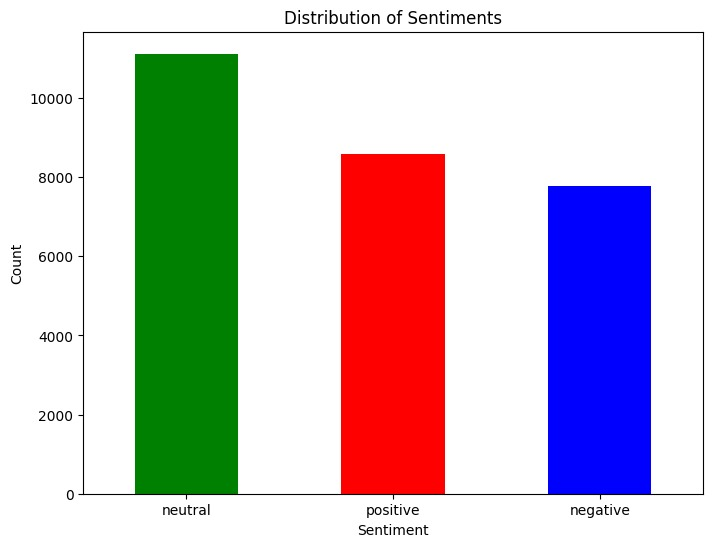
\includegraphics[width=\textwidth]{figs/5.jpg}
        \caption*{Sentiment Distribution}
        \label{fig:figure5}
    \end{minipage}
    
    \caption{Visualization of Correlation of features with Sentiments}
    \label{fig:dataset_figures}
\end{figure}
\begin{figure}[htbp]
    \centering
% First image
    \begin{minipage}[b]{0.3\textwidth}
        \centering
        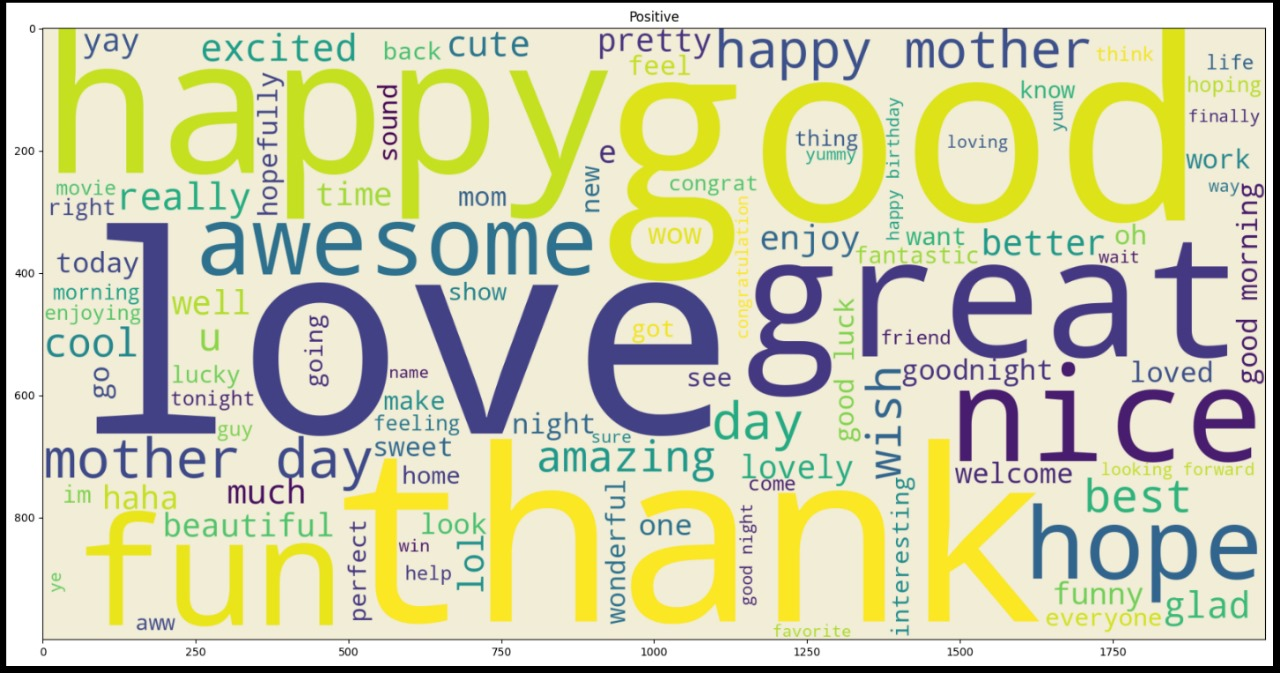
\includegraphics[width=\textwidth]{figs/positive.jpg}
        \caption*{Word Cloud for Positive Data}
        \label{fig:figure3}
    \end{minipage}
    \hfill
    % Second image
    \begin{minipage}[b]{0.3\textwidth}
        \centering
        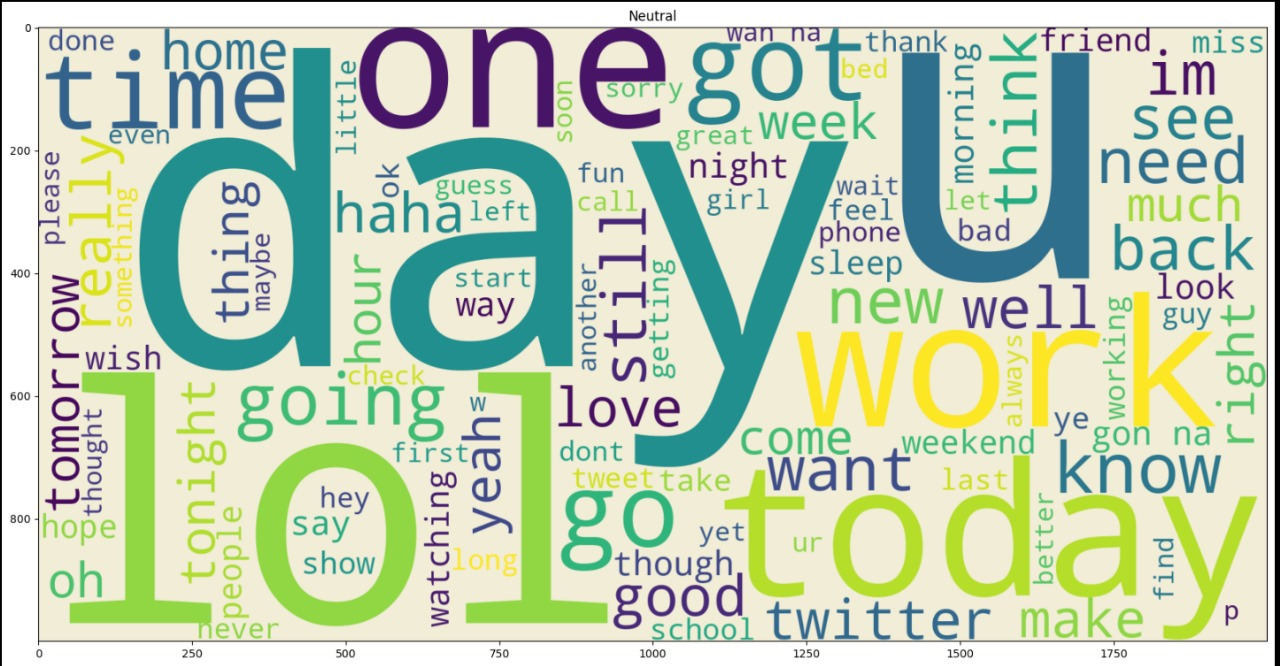
\includegraphics[width=\textwidth]{figs/nneutral.jpg}
        \caption*{Word Cloud for Neutral Data}
        \label{fig:figure4}
    \end{minipage}
    \hfill
    % Third image
    \begin{minipage}[b]{0.3\textwidth}
        \centering
        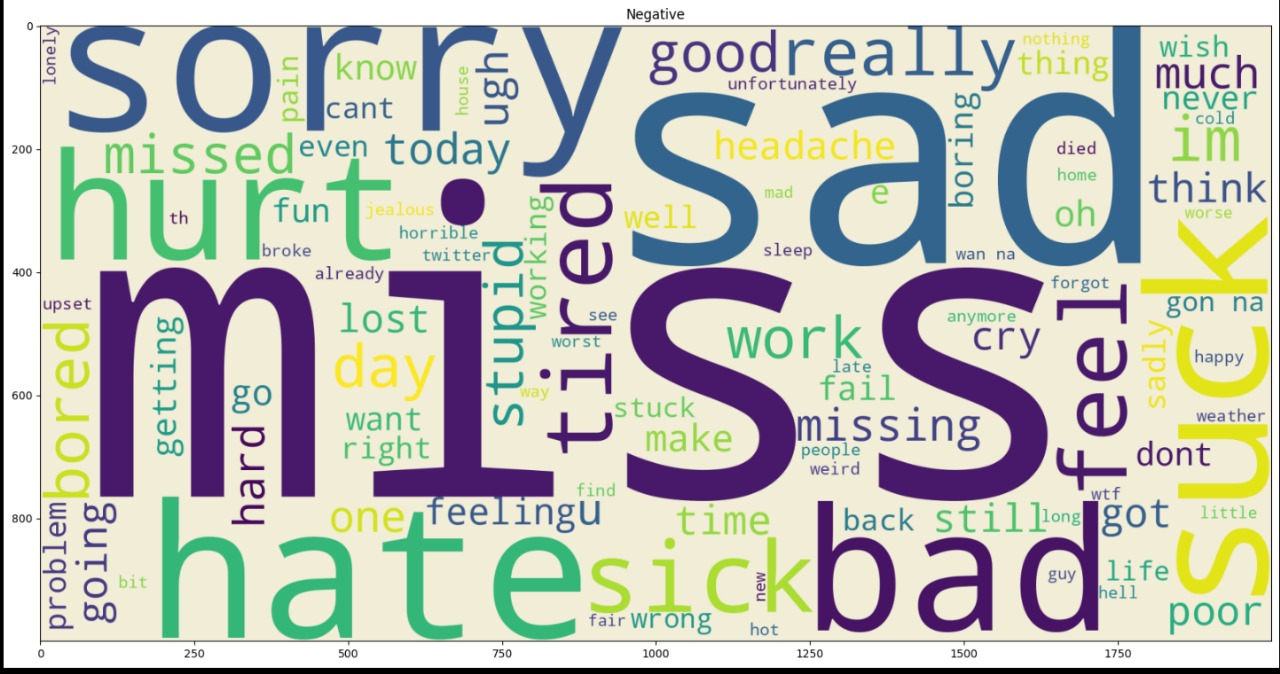
\includegraphics[width=\textwidth]{figs/neg.jpg}
        \caption*{Word Cloud for Negative Data}
        \label{fig:figure5}
    \end{minipage}
    \caption{Visualization of WordCloud for every sentiment}
    \label{fig:dataset_figures}
\end{figure}
\vspace{0.3 cm}
\begin{figure}[htbp]
    \centering
 % First image
    \begin{minipage}[b]{0.3\textwidth}
        \centering
        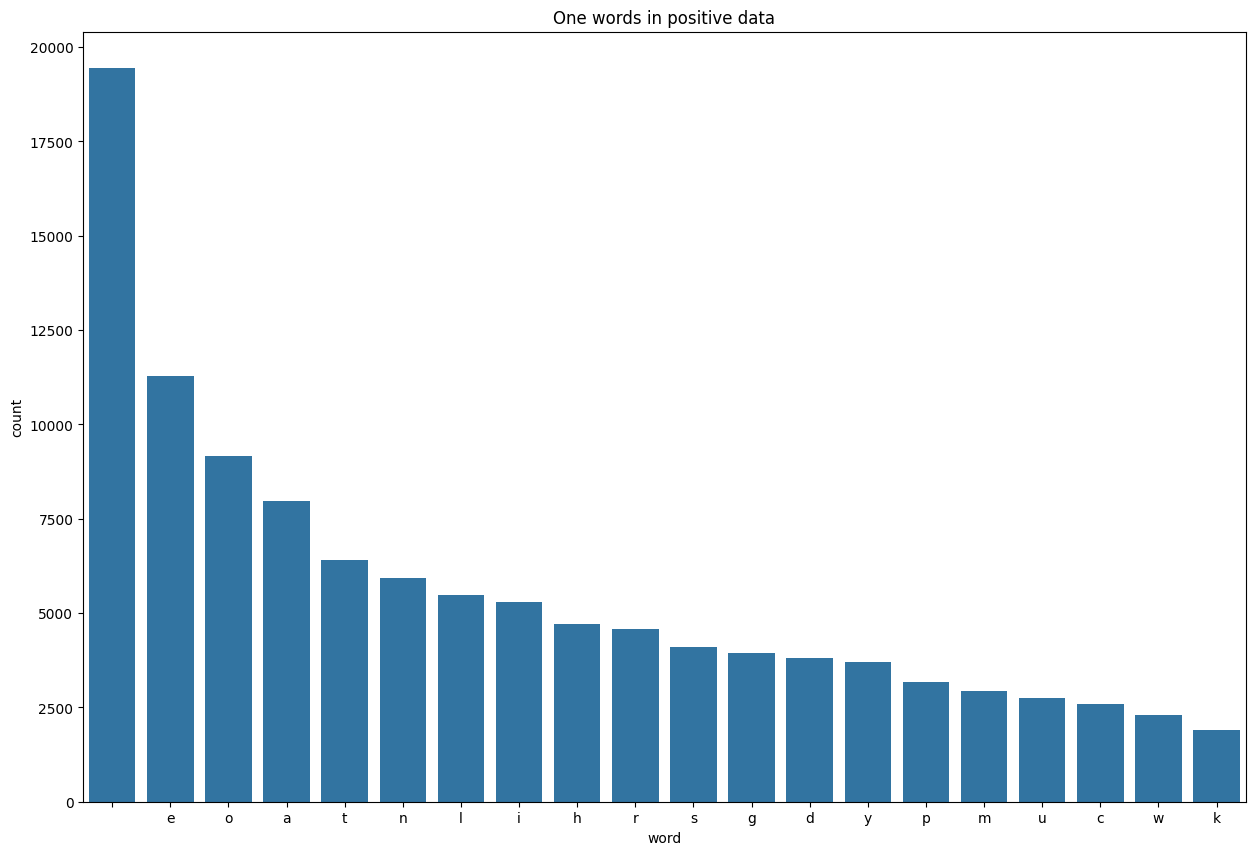
\includegraphics[width=\textwidth]{figs/output.png}
        \caption*{One word count for Positive Data}
        \label{fig:figure3}
    \end{minipage}
    \hfill
    % Second image
    \begin{minipage}[b]{0.3\textwidth}
        \centering
        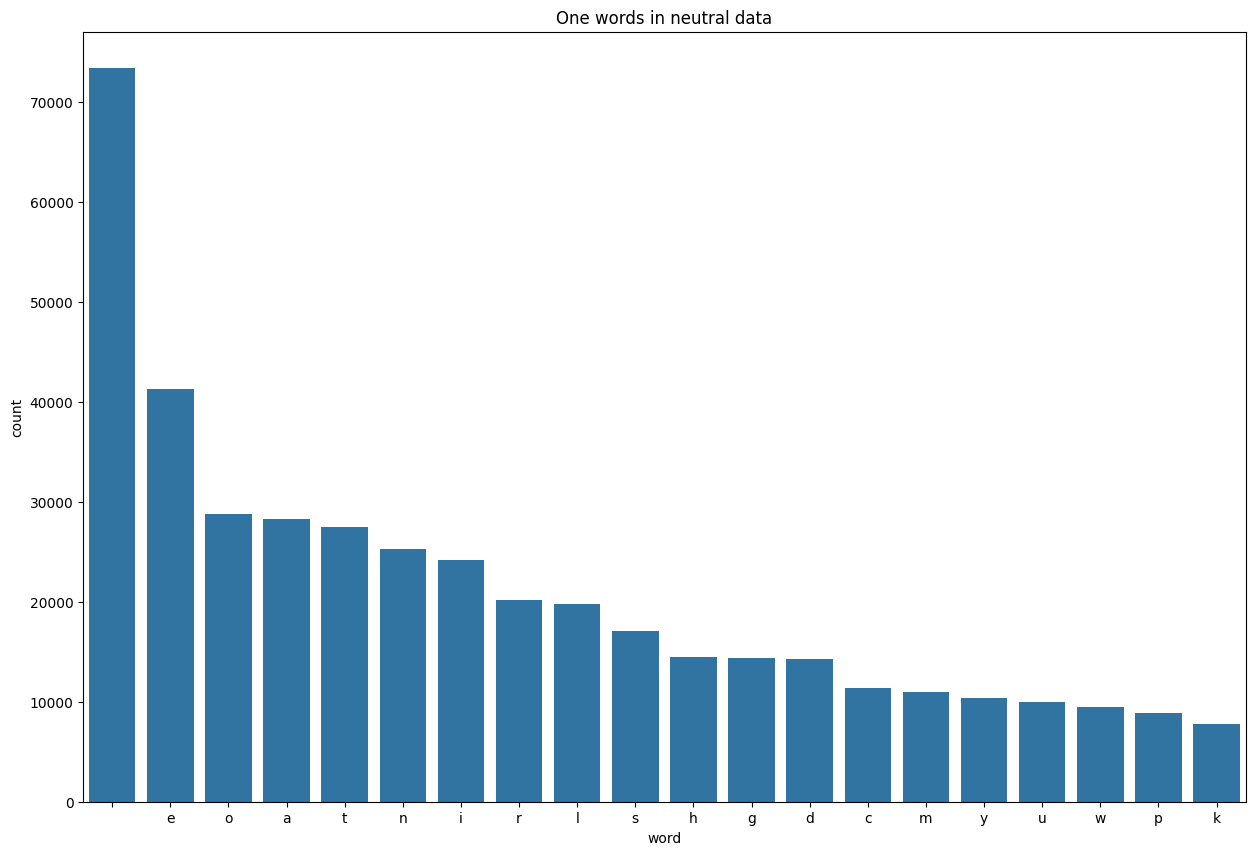
\includegraphics[width=\textwidth]{figs/output2.png}
        \caption*{One word count for Neutral Data}
        \label{fig:figure4}
    \end{minipage}
    \hfill
    % Third image
    \begin{minipage}[b]{0.3\textwidth}
        \centering
        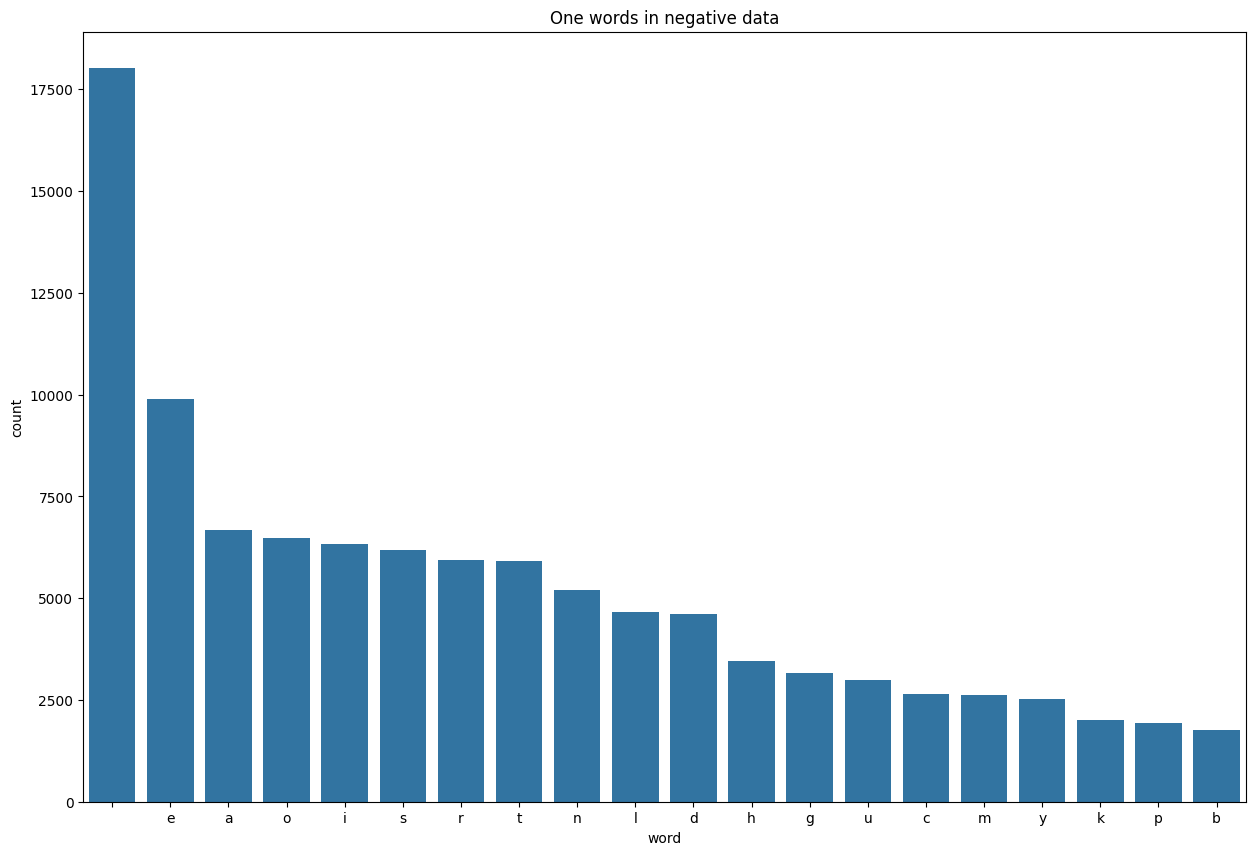
\includegraphics[width=\textwidth]{figs/output3.png}
        \caption*{One word count for Negative Data}
        \label{fig:figure5}
    \end{minipage}
    
    \caption{Visualization of One word count for every sentiment}
    \label{fig:dataset_figures}
\end{figure}

\begin{figure}[htbp]
    \centering
% First image
    \begin{minipage}[b]{0.3\textwidth}
        \centering
        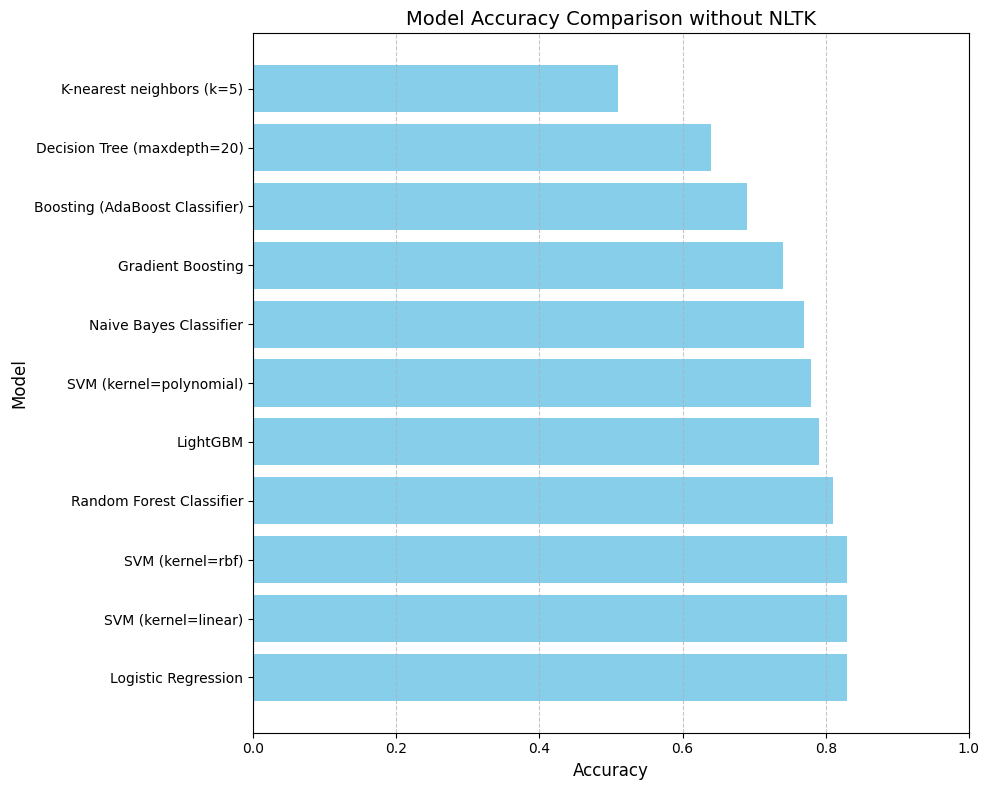
\includegraphics[width=\textwidth]{figs/download (2).png}
        \caption*{Model Accuracy Comparison without NLTK}
        \label{fig:figure3}
    \end{minipage}
    \hfill
    % Second image
    \begin{minipage}[b]{0.3\textwidth}
        \centering
        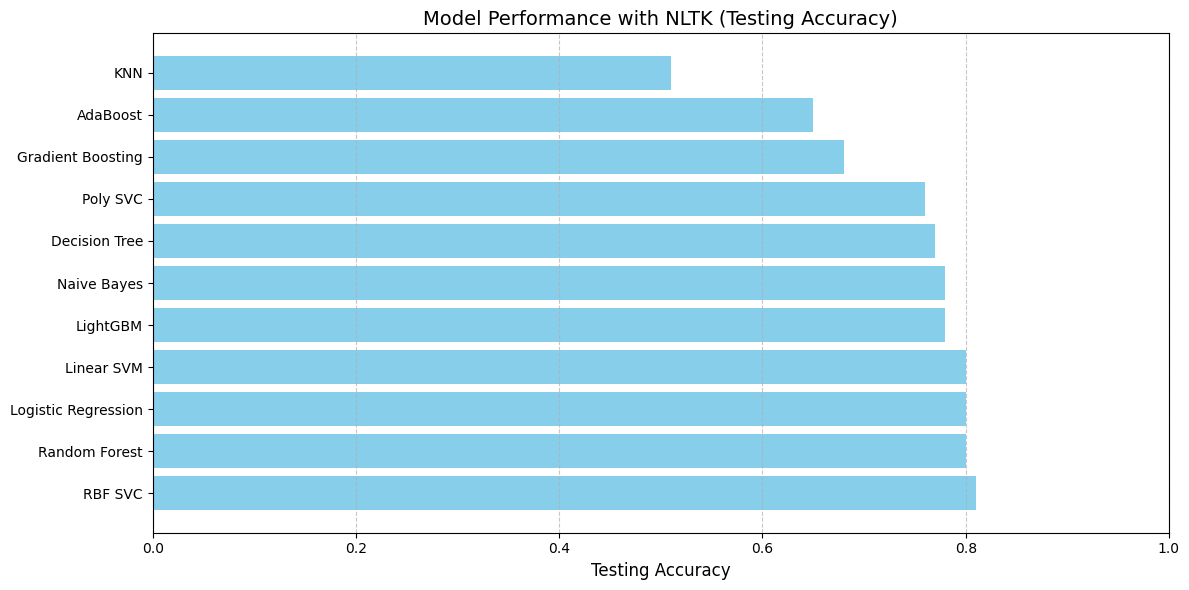
\includegraphics[width=\textwidth]{figs/download (3).png}
        \caption*{Model Testing Accuracy Comparison with NLTK}
        \label{fig:figure4}
    \end{minipage}
    \hfill
    % Third image
    \begin{minipage}[b]{0.3\textwidth}
        \centering
        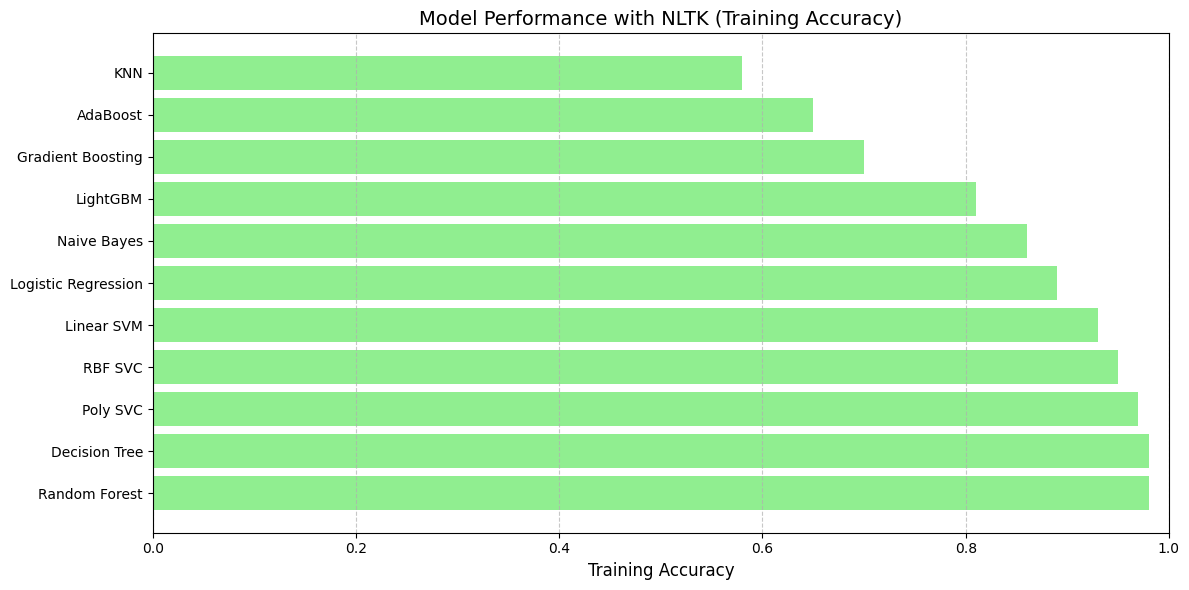
\includegraphics[width=\textwidth]{figs/download (4).png}
        \caption*{Model Training Accuracy Comparison with NLTK}
        \label{fig:figure5}
    \end{minipage}
    
    \caption{Visualization of Accuracy comparison over all the modes applied}
    \label{fig:dataset_figures}
\end{figure}
\cite{wang2014sentiment}
\cite{dang2020sentiment}
\cite{pang2002thumbs}
\cite{tang2014learning}
\bibliographystyle{ieeetr}  % Choose a bibliography style
\bibliography{refs}
	

\section{{Article References}}

\begin{itemize}
    
    \item \url{https://hp-analytics.medium.com/sentiment-analysis-solutions-and-applications-survey-9e52d3ea2ac7}
    \item \url{https://aman.ai/coursera-nlp/}\item \url{https://link.springer.com/article/10.1007/s10462-022-10144-1}
    \item \url{https://scikit-learn.org/stable/modules/tree.html}
    \item \url{https://www.analyticsvidhya.com/blog/2021/08/decision-tree-algorithm/}
    \item \url{https://www.simplilearn.com/gradient-boosting-algorithm-in-python-article}
    \item \url{https://www.analyticsvidhya.com/blog/2021/09/adaboost-algorithm-a-complete-guide-for-beginners/}
    \item \url{https://www.ibm.com/topics/knn}
    \item \url{https://www.analyticsvidhya.com/blog/2021/08/complete-guide-on-how-to-use-lightgbm-in-python/}
\end{itemize}

	\appendix
	
	\section{Contribution of each member}
	\label{sec:contribution}
	\begin{enumerate}
	\item \textbf{Mahek Vanjani:} Implemented \textbf{Decision Tree} and explored various preprocessing steps, including word embeddings, which resulted in low accuracy. Contributed to creating a \textbf{GitHub repository }with well-written code and a proper readme file. Also played a major role in \textbf{drafting the report}, analyzing research papers, and contributing to the \textbf{presentation} and video formation.
	\item \textbf{Himanshu Sharma:} Implemented \textbf{Naive bayes} and explored various preprocessing steps.I played a pivotal role in designing and developing the \textbf{project's web page}. Leveraging my proficiency in web development technologies such as HTML, CSS, and JavaScript, I created an intuitive and user-friendly interface. The web page serves as a central hub for accessing project resources, including data sets, code repositories, and documentation, enhancing accessibility.Played a major role in \textbf{research of selecting algorithms} for the project.
	\item \textbf{Priyansh Saxena:} Implemented \textbf{Support Vector Machine (SVM)}. Aggregated and combined all the algorithms in the \textbf{NLTK implementation}. I played an important role in designing and developing the \textbf{Project's Web Demo}. I deployed the interactive web demo on Hugging Face spaces using Gradio. Also, demonstrated the web demo in the youtube video. The web demo serves as a way for users to use and interact with the model in real time.
    \item \textbf{Vasishtha Pandya:} Implemented \textbf{ Random Forest and boosting methods}. Implemented the following boosting methods : Adaboost, Gradient Boosting Machine (GBM), and LightGBM. Explored the preprocessing steps in \textbf{NLTK implementation}. Played a major role in research of selecting algorithms for the project. Contributed in youtube video formation of results.
    \item \textbf{Saumya Shah:} Contributed in making the webpage of project. Also contributed in making presentation for the youtube video.Also being a active member during discussions on project,and gave useful suggestions for the project duration.
    \item \textbf{Vidhi Jain:} Contributed in making the report of project. Also implemented KNN model.Also being a active member during discussions on project,and gave useful suggestions for the project duration.
    \item \textbf{Anushka Desai:} Contributed in the formation  video of project.Also implemented Logistic Regression model and tried it using various parameters.Also helped in forming of the presentation.
    
    
    \end{enumerate}
 
\end{document}


